\section{Auswertung}
Zur Bestimmung der Parameter der Probe ist es zunächst notwendig den Geometriefaktor $G$:
\begin{equation}
  G =
     \begin{cases}
       \frac{D}{\sin\left(\upalpha_i\right)}{d_0} &\quad\upalpha_i<\upalpha_g\\
       1 &\quad\upalpha_i\geq\upalpha_g
     \end{cases}
\end{equation}
zu berechnen. Hierbei ist $\upalpha_i$ der Einfallswinkel der Strahlung auf die Probe und $\upalpha_g$ der Geometriewinkel
\begin{equation}
\upalpha_g=\arcsin(\frac{d_0}{D}).
\end{equation}
$D=2\,\si{\cm}$ ist der Probendurchmesser und $d_0=0{,}2\,\si{\mm}$ die Höhe des Strahls. Der Geometriewinkel wird während des Justierens bestimmt und ist in diesem Fall $\upalpha_g=0.5717°$.
Durch Teilen der Messwerte durch den Geometriefaktor wird berücksichtigt, dass erst ab ausreichend großen Winkeln der gesamte Strahl die Probe trifft. Messwerte für sehr flache Winkel werden ausgelassen, da hierbei die Strahlung noch direkt in den Detektor treffen kann.\\
Zur Aufbereitung der Daten werden außerdem die Messdaten der Diffusionsmessung von denen der direkten Reflektionsmessung abgezogen. Zum Darstellen der aufgenommenen Messwerte werden die aufgenommenen Daten gegen den Wellenvektorübertrag $q_z=\frac{4\pii}{\lambda}\sin(\upalpha_i)$ aufgetragen. Hierbei ist $\lambda$ die Strahlungswellenlänge von $1{,}54\cdot10^{-10}\,\si{\m}$. Die Ergebnisse sind in Abb.\ref{Plot1} zu sehen.
\begin{figure}[H]
  \centering
  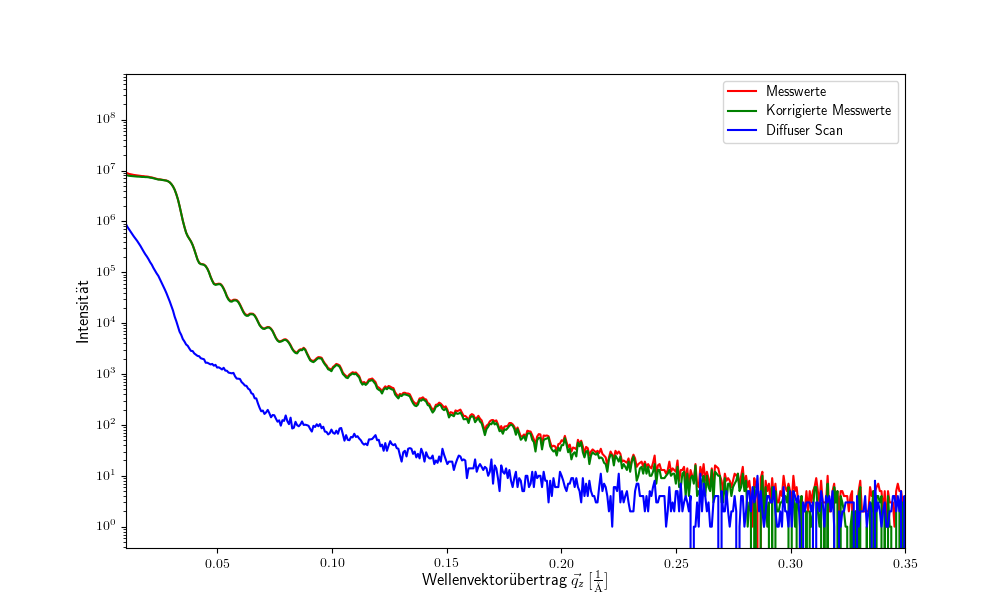
\includegraphics[width=\textwidth]{Berechnung/Plot1.png}
  \caption{Reflektivitätsscan aufgetragen gegen den Wellenvektor.}
  \label{Plot1}
\end{figure}
\subsection{Bestimmung der Probenparameter}
Zur Bestimmung der Probenparameter wird der Parratt-Algorithmus genutzt, um eine Theoriekurve an die  korrigierten Messwerte anzupassen. Die Schichtdicke $d$ lässt sich gemäß:
\begin{equation}
d=\frac{2\pi}{\upDelta q_z}
\end{equation}
bestimmen, indem die Periodendauer zwischen zwei Maxima vermessen wird. Durch die Lage des kritischen Winkels der Totalreflexion lässt sich danach der Brechungsindex des Substrates bestimmen. Die restlichen Parameter werden solange variiert, bis eine optimale Anpassung an die Messwerte erreicht wird. Hier ergibt sich für die Parameter damit:
\begin{align}
  \text{Brechungsindex Luft}:&\quad n_\text{Luft}=1\\
  \text{Brechungsindex Schicht}:&\quad n_\text{Schicht}= \left(1-1,2\right)\cdot10^{-6}\\
  \text{Brechungsindex Substrat}:&\quad n_\text{Substrat}=\left(1-7,4\right)\cdot10^{-6}\\
  \text{Rauigkeit Schicht}:&\quad \upsigma_\text{Schicht}=\left(15,5\right)\cdot10^{-10}\\
  \text{Rauigkeit Substrat}:&\quad \upsigma_\text{Substrat}=\left(9,8\right)\cdot10^{-10}\\
  \text{Schichtdicke}:&\quad z=873\,\AA
\end{align}
Die Kurve der korrigierten und normierten Messwerte sowie die des Parratt-Algorithmus sind in Abb.\ref{fit} dargestellt.
\begin{figure}[H]
  \centering
  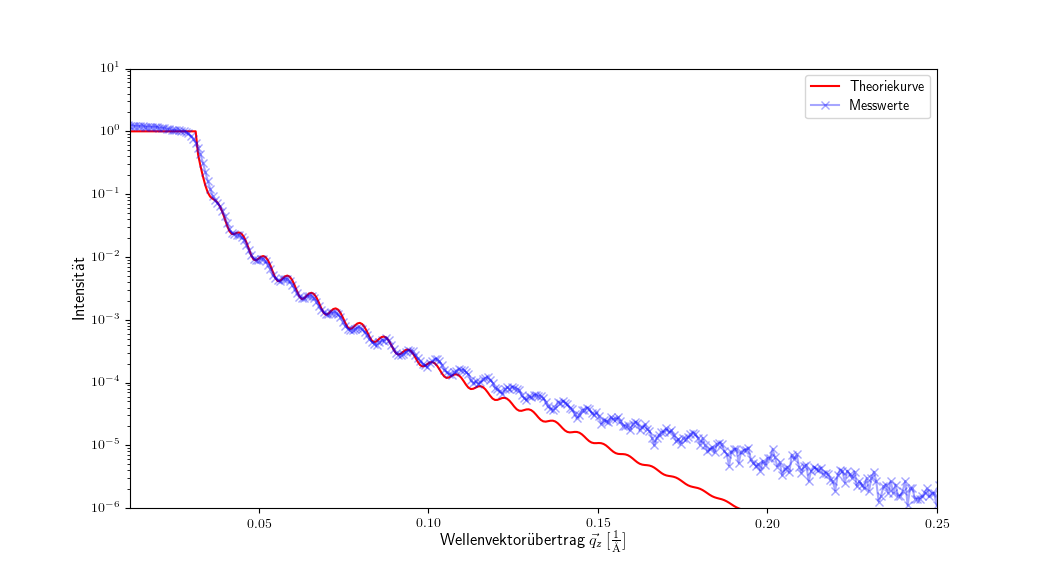
\includegraphics[width=\textwidth]{Berechnung/Fit.png}
  \caption{Kurve des Parratt-Algorithmus angepasst an die Messwerte.}
  \label{fit}
\end{figure}
